\chapter{Verwandte Arbeiten}\label{chapter:arbeiten}
In diesem Kapitel werden verwandte Arbeiten betrachtet, die sich mit der Forschungsfrage \glqq Wie lassen sich die Konzepte der Augmented Reality für den Bildungsbereich nutzen?\grqq{} oder einer angrenzenden Thematik beschäftigen. Dabei wird sowohl auf allgemeine Literatur, Studien, wissenschaftliche Arbeiten, als auch konkrete Anwendungen eingegangen und ihr Inhalt zusammengefasst.


\section{Augmented Reality in der Bildung}
Im folgenden werden Veröffentlichungen betrachtet, die sich mit dem Einsatz von Augmented Reality beschäftigen. Zum Teil beleuchteten die Arbeiten konkrete Einsatzmöglichkeiten von Augmented Reality, zum anderen werden die Vorteile von Augmented Reality oder Richtlinien für AR-Anwendungen betrachtet.


\subsection{Geroimenko: Augmented Reality in Education}
Das Buch \glqq Augmented Reality in Education\grqq{} von \citeauthor{geroimenko:ar-in-education} beschäftigt sich mit den Grundlagen des Einsatzes von Augmented Reality im Bildungsbereich. Dabei wird auf den aktuellen Stand, die aktuellen Einsatzbereiche, aber auch auf die konkrete Entwicklung von AR-Anwendungen für den Bildungsbereich eingegangen. 

\subsubsection{Zusammenfassung}
Insgesamt lassen sich die Aussagen des Buches wie folgt zusammenfassen:
\subparagraph{Aktueller Stand}
Smartphones stellen aufgrund des Vorhandenseins verschiedener Software Development Kits (SDK) und ihrer Allgegenwart die aktuelle Hauptplattform für Augmented Reality dar. Während Head Mounted Displays vor allem an kleinere Zielgruppen und den professionellen Markt richten. \citep[Kapitel 1.2]{geroimenko:ar-in-education}\\
\begin{figure}
\centering
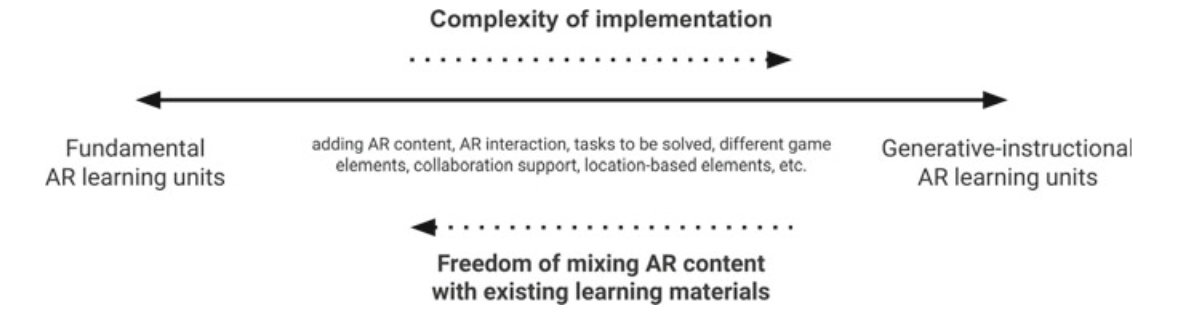
\includegraphics[width=1.0\textwidth]{Abbildungen/ar-object-continuum.png}
\caption[Komplexitätskontinuum von AR-Objekten]{Das Komplexitätskontinuum von AR-Objekten. (Quelle: \cite[S. 9]{geroimenko:ar-in-education})}
\label{fig:komplexitätskontinuum}
\end{figure}
Generell kann bei AR-Objekten zwischen fundamentalen und generativen AR-Lerneinheiten unterschieden werden, die jeweils ein Ende eines Kontinuums darstellen (vergleiche Abbildung \ref{fig:komplexitätskontinuum}).
Der ausschlaggebende Faktor ist dabei die Komplexität des Objektes, je höher diese ist, desto generativer ist die Lerneinheit, aber umso geringer ist die Möglichkeit die AR-Inhalte mit den existierenden Lerninhalten zu verbinden. 
Generative AR-Lerneinheiten stehen dementsprechend mehr für sich alleine und decken ein größeres inhaltliches Feld ab.
Der Zugriff auf diese fundamentalen AR-Inhalte ist heutzutage bereits sehr einfach und die Entwicklung in der Thematik wird sich vermutlich ähnlich analog zu der Entwicklung der VR-Inhalte, bei welcher die generative Inhalte nach und nach hinzukamen, verhalten.\citep[Kapitel 1.3]{geroimenko:ar-in-education}\\
Die aktuelle Hauptzielgruppe im schulischen Bereich ist dabei die weiterführende Schule. Außerhalb des schulischen Umfeldes kann AR zur Ausbildung von Fachkräften eingesetzt werden. \citep[Kapitel 1.5]{geroimenko:ar-in-education}

\subparagraph{Entwicklung von Augmented Reality Anwendugen}
Vor der Entwicklung einer Augemented Reality Anwendung für den Bildungsbereich, sollten folgende Entscheidungen getroffen werden:
\begin{enumerate}
\item Die erste Entscheidung, die bei der Entwicklung getroffen werden muss, bezieht sich auf die eingesetzte Technologie. Dabei muss überlegt werden, welche Geräte die Schüler bereits besitzen und welche alternativ angeschafft werden könnten. Des weiteren muss bedacht werden, dass auch die Lehrenden im Umgang mit den neuen Technologie geschult werden müssen.
\item Als Zweites muss überlegt werden, was durch den Einsatz der Anwendung erreicht werden soll. Dabei muss grundsätzlich zwischen fundamentalen Lerneinheiten, die angeschaut und vom Nutzer manipuliert werden können, und generativen, instruktiven Lerneinheiten, welche verschiedenen Interaktionsmöglichkeiten, Spielelemente, Beteiligungsformen und vieles mehr enthalten,  abgewogen werden. 
\item Des Weiteren muss bedacht werden, dass für die Erstellung von AR-Lernobjekten unter Umständen komplexe Fähigkeiten notwendig sind. Während einfache, dreidimensionale Objekte anhand von Bildern realer Objekte generiert werden können, ist die Erstellung komplexer Lerninhalte aufgrund mangelnder Werkzeuge sehr aufwendig und erfordert weitere Spezialkräfte.
\item Der letzte Punkt ist die Zielgruppe. Hier muss zwischen einem breitem Feld an Einsatzgebieten, wie Schulen, Museen und vielem mehr, abgewogen werden, da sich die Anforderungen der Teilgebiete stark unterscheiden können. 
\end{enumerate}
\citep[Kapitel 1.7]{geroimenko:ar-in-education}

\subparagraph{Augmented Reality in der Lehre}
In der Lehre kann Augemented Reality ein breites Feld bedienen.\\
Ein Einsatzbereich stellen dabei die Naturwissenschaften und die Medizin dar.
Besonders Letzteres kann von Augmented Reality in den folgenden Bereichen profitieren:
\begin{itemize}
\item Anatomie: Hierbei kann AR von Medizinstudenten dazu genutzt werden die Anatomie des Körpers besser zu verstehen, indem sie 3D Modelle im AR-Bereich bertrachten können.
\item Mentoring: Mit Hilfe von AR ist es möglich das Studenten Prozeduren kennenlernen und erfahren, in denen sie noch nicht geschult sind. 
\item Klinische Fertigkeiten: Auch die klinischen Fähigkeiten der Studenten können verbessert werden, indem mit der Hilfe von Augmented Reality klinische Simulationen durchgeführt werden.
\end{itemize}
\citep[Kapitel 7-9]{geroimenko:ar-in-education} \\
Augmented Reality kann zudem für die Umweltbildung im Freien genutzt werden. Dabei bietet AR die Möglichkeit die Komplexität der Umgebung aus verschiedenen Perspektiven zu visualisieren, detaillierte und wissenschaftliche Informationen anzuzeigen oder das \glqq Unsichtbare\grqq{} sichtbar zumachen.
Dabei ermöglicht es dem Lernenden eine andere Perspektive auf das Sichtbare, in dem es Parameter, wie die Zeit (Vergangenheit, Zukunft), die Skalierung (mikroskopische Sicht, Vogelperspektive) oder die Wahrnehmbarkeit (Unsichtbares enthüllen, Sichtbares verdecken), verändert. \citep[Kapitel 17]{geroimenko:ar-in-education}\\
Auch in Bereichen der Archäologie kann AR als Forschungsinstrument für die Rekonstruktion und Interpretation eingesetzt werden. \citep[Kapitel 17]{geroimenko:ar-in-education}\\
Ein weiterer Bereich, den Augmented Reality abdecken kann, sind die Geisteswissenschaften.
Hier stellt die Erweiterung der Umgebung basierend auf der aktuellen Position des Nutzers durch AR eine wichtige Einsatzmöglichkeit dar. Dadurch lassen sich beispielsweise Zusatzinformationen zu historischen Gebäuden anzeigen und es ist möglich dem Nutzer einen Eindruck zu vermitteln wie ein Ort in der Vergangenheit einmal aussah. \citep[Kapitel 11-12]{geroimenko:ar-in-education}\\
Im Bereich des Lernens einer Fremdsprache, bietet AR die Möglichkeit das konventionelle Lernen im Klassenzimmer um eine virtuelle Welt erweitern, um die Motivation der Lernenden zu steigern. \citep[Kapitel 11-12]{geroimenko:ar-in-education}

\subparagraph{Konkrete Anwendungsbeispiele}
Das FeDiNAR-Projekt stellt ein konkretes Anwendungsbeispiel der Augmented Reality zur Ausbildung von Personen dar. Es hat das Ziel, die Fehler mit Hilfe von Augmented Reality zu einer Lernmöglichkeit umzuwandeln. Das Konzept beruht darauf Fehler nicht durch den Ausbilder zu verhindern, sondern sie zuzulassen. Dieses soll möglich sein, indem die Auszubildenden zwar an echten Maschinen arbeiten, die Auswirkungen ihrer Handlungen dabei jedoch lediglich in der Augmented Reality dargestellt werden. 
\citep[Kapitel 5]{geroimenko:ar-in-education}\\
Ein weiteres kleines Projekt ist die im Rahmen des Buches beschriebene Entwicklung einer Online-Plattform zur verbesserten Lernerfahrung. Die Anwendung beruht auf \glqq durchsichtige\grqq{} Markern, die in ein Bild eingefügt werden konnten. Wurde der Marker innerhalb eines Bildes erkannt wird ein dreidimensionales Modell des Bildes mit Hilfe von Augmented Reality angezeigt. \citep[Kapitel 3]{geroimenko:ar-in-education}

\subsubsection{Relevanz für dieses Arbeit}
Das Buch von \citeauthor{geroimenko:ar-in-education} gibt einen ersten Überblick über Augmented Reality in der Bildung und deren mögliche Einsatzszenarien. Vor allem die Richtlinien bei der Entwicklung von Augmented Reality Anwendungen zu Bildungszwecken sollten in den folgenden Kapiteln berücksichtigt werden.  


\subsection{Hedberg: A Systematic Review of Learning through Mobile Augmented Reality}\label{sec:hedberg-review}
In der wissenschaftlichen Arbeit \glqq A Systematic Review of Learning through Mobile Augmented Reality\grqq{} aus dem Jahr \citeyear{hedberg:review-ar-learning} von \citeauthor{hedberg:review-ar-learning} wurde mit Hilfe einer systematischen Literaturauswertung eine Einschätzung des Einsatzes von Augmented Reality zu Bildungszwecken vorgenommen. \\
Dabei wurde die Relevanz einzelner Einsatzgebiete anhand der Anzahl an Veröffentlichungen zum jeweiligen Thema gemessen.\\ Die Veröffenntlichungen stammen dabei aus den Datenbanken \glqq IEEE Xplore\grqq , \glqq Elsevier\grqq{} und der \glqq ACM digital libary\grqq{} und wurden über Schlüsselwörter herausgesucht. Die Ergebnisse der Suche wurden im Anschluss noch gefiltert und kategorisiert, um irrelevante Veröffentlichungen auszuschließen.

\subsubsection{Zusammenfassung}
Anhand der gesammelten wissenschaftlichen Arbeiten kam die Studie von \citeauthor{hedberg:review-ar-learning} zu den folgenden Ergebnissen in den für diese Arbeit relevanten Kategorien:

\subparagraph{Bildungsniveau}
Diese Kategorie zielte darauf ab die Zielgruppen der AR-Systeme herauszufinden. Dabei kam die Studie zu dem Ergebnis, dass die meisten Systeme (fast 50 \%) bezogen auf das amerikanische Bildungssystem für die Universität geschaffen wurden. Mit einem deutlichen Abstand folgt die Grundschule, die Junior High School, die High School und die Vorschule. \citep[S. 78]{hedberg:review-ar-learning}

\subparagraph{Mobiles Endgerät}
In dieser Kategorie ging es darum herauszufinden welches die meist genutzten Endgeräte für Augmented Reality im Bildungsbereich darstellen. Hierbei kam heraus, dass das Handy bzw. das Smartphone (43,84 \%) gefolgt von dem Tablet (27,40 \%) diese Kategorie dominieren, wobei ebenfalls 27 \% der wissenschaftlichen Arbeiten keine spezifische Plattform angaben. \citep[S. 80]{hedberg:review-ar-learning}

\subparagraph{Unterrichtsfach}
Diese Kategorie untersuchte die fachliche Ausrichtung der Augmented Reality und kam zu dem Ergebnis, dass die Systeme vor allem in den Naturwissenschaften genutzt werden. Darauf folgen mit signifikantem Abstand die Sprachen, Geschichte und Technik. \citep[S. 81]{hedberg:review-ar-learning}

\subparagraph{Lernerfolge}
Hierbei wurden Studien untersucht, die sich mit dem pädagogischen Nutzen von Augmented Reality beschäftigt haben. Dabei kamen von 73 Studien lediglich zwei nicht zu dem Ergebnis, dass AR einen positiven Einfluss auf das Lernen besitzt.\\
Allgemein stellten 45 Veröffentlichungen (54,88 \%) eine erhöhte Motivation und ein verbessertes Engagement fest. 28 Studien (34,15 \%)konnten verbesserte Lernergebnisse bei den Studenten aufzeigen.  \citep[S. 81-82]{hedberg:review-ar-learning}

\subparagraph{Pädagogische Methoden}
In der letzten Kategorie, wurden die Einsatzarten von Augmented Reality im Bildungsbereich untersucht und das Ergebnis erarbeitet, dass die drei Hauptanwendungsmethoden das interaktive, das forschungsbasierte und das kollaborative Lernen sind. \citep[S. 82]{hedberg:review-ar-learning}

\subsubsection{Relevanz für diese Arbeit}
Die Ergebnisse der Studien geben einen ersten Einblick in die Fragestellung, wie Augmented Reality in der Bildung bereits genutzt wird. In den folgenden Kapiteln muss einerseits überlegt werden, in welchen Bereichen der zu entwickelnde Anwendungsfall und Prototyp an den aktuellen Stand anknüpfen soll. Anderseits muss abgewogen werden, an welchen Stellen eine eventuell eine Nische, die durch die Forschung und die aktuellen Anwendungen bisher kaum beziehungsweise gar nicht behandelt wird, abgedeckt werden soll.


\subsection{Billinghurst: Augmented Reality in Education}\label{sec:billinghurst-ar-education}
\citeauthor{billinghurst:ar-in-education} untersuchte in seiner Veröffentlichung \glqq Augmented Reality in Education\grqq{} aus dem Jahr \citeyear{billinghurst:ar-in-education} den Einsatz von Augmented Reality im Bildungsbereich.\\

\subsubsection{Zusammenfassung}
In der Veröffentlichung stellt \citeauthor{billinghurst:ar-in-education} drei grundlegende Eigenschaften der Augmented Reality im Bildungsbereich heraus.

\subparagraph{Interaktion}
\citeauthor{billinghurst:ar-in-education} führt hier auf, dass Schüler besser zusammenarbeiten, wenn sie sich gemeinsam auf einen Arbeitsplatz fokussieren. Dieses ist bei computerbasierten Lernen schwierig umzusetzten, da sich jeder auf den Bildschirm vor sich konzentriert. Dadurch fehlt eine wichtige Eigenschaft, welche die Kommunikation in der Gruppe verbessert: die gegenseitige Sichtbarkeit. Wenn Schüler gleichzeitig das Objekt der Diskussion und ihre Diskussionspartnern sehen, werden auch die nichtverbalen Gesprächsmerkmale, wie Gesten oder die Mimik wahrgenommen. Diese Merkmale bilden einen essentiellen Teil der menschlichen Kommunikation. 
Durch den Einsatz von Augmented Reality können diese Eigenschaften beibehalten werden und trotzdem gleichzeitig computerbasierte Inhalte angezeigt werden. \citep[S. 2-3]{billinghurst:ar-in-education}

\subparagraph{Greifbare Schnittstelle}
Hier führt \citeauthor{billinghurst:ar-in-education} auf, dass im Bildungsbereich physische Objekte dazu genutzt werden Bedeutung von theoretischem Wissen zu übermitteln, in dem sie die Eindrücke des Schülers, durch ihre Erscheinung, ihre physikalischen Eigenschaften, ihren räumlichen Beziehungen und der Fähigkeit, die Aufmerksamkeit zu fokussieren, verstärken.\\
Diese Eigenschaften lassen sich zu großen Teilen auch auf die virtuellen Objekte in der Augmented Reality beziehen. Auf Grund der direkten Beziehungen zwischen den virtuellen Objekten und der Augmented Reality ist zum Beispiel eine physikalisch basierte Interaktion mit den computergenerierten Objekten möglich. \citep[S. 3]{billinghurst:ar-in-education}

\subparagraph{Übergangsschnittstelle}
Im dritten Abschnitt bezieht sich \citeauthor{billinghurst:ar-in-education} auf das bereits in Kapitel \ref{sec:ar} eingeführte RV-Kontinuum und führt an, dass man mittels AR den Nutzer entlang des Kontinuums in die virtuelle Welt führen kann. Besonders Kinder können so in die Seiten eines Buches eintauchen und die Fantasie Realität werden lassen. Dadurch werden aus statischen Unterrichtsbüchern dynamische interaktive Umgebungen. \citep[S. 3-4]{billinghurst:ar-in-education}

\subsubsection{Relevanz für diese Arbeit}
\citeauthor{billinghurst:ar-in-education} führt in seiner Veröffentlichung drei wichtige Eigenschaften zum Einsatz von Augmented Reality im Bildungsbereich auf, die im weiteren Verlauf der Arbeit bedacht werden sollten. Zum einen sollte eine AR-Anwendug nicht dafür sorgen, dass die Umgebung ausgeblendet wird, sondern die Anwendung sollte diese erweitern und ein Bewusstsein des Umfeldes schaffen. Zum anderen ist die Darstellung der Lerninhalte im Raum und ihrer Eigenschaften ein wichtiger Faktor, um den Nutzen der Augmented Reality vollends auszuschöpfen. 


\subsection{Diegmann: Benefits of Augmented Reality in Educational Environments}\label{sec:diegmann-benefits-ar}
In dem Artikel \glqq  Benefits of Augmented Reality in Educational Environments\grqq{} von \citeauthor{diegmann:benefits-ar} aus dem Jahr  \citeyear{diegmann:benefits-ar} werden die Vorteile der Augmented Reality für den Bildungsbereich betrachtet. \\
Dabei wurde eine systematische Evaluation von Augmented Reality anhand der Veröffentlichungen zu diesem Thema durchgeführt. \\

\subsubsection{Zusammenfassung}
Basierend auf der Literatur stellte der Artikel zunächst in den folgenden Bereichen positive Effekte der Augmented Reality fest und ordnet sie anschließend bestimmten Anwendungsarten zu.

\subparagraph{Verfassung}
In verschiedenen Veröffentlichungen wurde eine Verbesserung der Motivation festgestellt. Dieses umfasst ein erhöhtes Engagement und Interesse gegenüber den Lerninhalten und der Technologie.\\
Des weiteren wurde auch eine Steigerung der Aufmerksamkeit und der Konzentration, bezogen auf die Inhalte mit denen die Lernenden konfrontiert wurden, festgestellt.\\
Zu dem verbesserte sich auch die Zufriedenheit der Schüler bezüglich der Bildungsfortschritte und des Lernprozesses. 
\citep[Kapitel 4.1]{diegmann:benefits-ar}

\subparagraph{Lehrkonzept}
Das Lehrkonzept verbessert sich durch AR  dahingehend, dass ein schülerzentriertes Lernen ermöglicht, wodurch das unabhängige, eigenverantwortliche Lernen der Schüler, sowie die Fähigkeit Wissensinhalte aufzunehmen verbessert wird.\\
Auch eine Verbesserung des kollaborativen Lernens kann durch AR erreicht werden. Dabei kann Schülern durch AR die Möglichkeit zur gemeinsamen Problemlösung und Kommunikation gegeben werden.
\citep[Kapitel 4.2]{diegmann:benefits-ar}

\subparagraph{Darstellung}
Auch die Darstellung von Lerninhalten kann mit Hilfe von AR-Anwendungen verbessert werden. So können AR-Inhalte einen höheren Detailgrad ermöglichen und die Zugänglichkeit von Lerninhalten und die Interaktivität mit diesen Inhalten verbessern. Besonders die neuen Interaktionsmöglichkeiten unterstützen ein Lernen durch eigene Erfahrungen.
\citep[Kapitel 4.3]{diegmann:benefits-ar}

\subparagraph{Lerntyp}
Ein weiterer Vorteil ist die Verbesserung der Lernkurve dar. Schüler, die mit Hilfe von Augmented Reality Unterrichtsinhalte erfassen konnten, lernten schneller und einfacher als Schüler ohne diese Möglichkeit.\\
Auch eine Verbesserung der Kreativität, der Wissensaufnahme und der Problemlösung konnte in verschiedenen Veröffentlichungen festgestellt werden.
\citep[Kapitel 4.4]{diegmann:benefits-ar}

\subparagraph{Verständnis}
Dieser Bereich bezieht sich auf das Wissen, das durch Augmented Reality erlangt werden kann.\\
Dabei kann, neben einem deutlich gesteigertem räumlichen Verständnisses, auch eine Steigerung des Gedächtnisses beobachtet werden. So konnten Schüler mit Hilfe von AR sich besser an Inhalte erinnern. \\
\citep[Kapitel 4.5]{diegmann:benefits-ar}

\subparagraph{Vorteile der verschiedenen Anwendungsarten}
Diese zuvor definierten Vorteile ordnen \citeauthor{diegmann:benefits-ar} auf Basis der Literatur den folgenden Anwendungsarten zu:
\begin{itemize}
\item Entdeckungsbasiertes Lernen: Bei entdeckungsbasierten Anwendungen erhält der Benutzer \glqq Informationen über einen realen Ort, während er gleichzeitig das interessierende Objekt betrachtet\grqq{} \citep[Kapitel 2.2]{diegmann:benefits-ar} \\
Bei Art von Anwendungen konnte vor allem eine Verbesserung der Lernkurve und des Geisteszustandes bei den Lernenden beobachtet werden. Insgesamt deckt diese Kategorie die meisten Vorteile im Vergleich zu den anderen Anwendungsarten ab. \citep[Kapitel 5]{diegmann:benefits-ar}
\item Objektmodellierung: Diese Gruppe beschreibt Modellierungsanwendungen, die mit Hilfe von Augmented Reality dem Nutzer direktes Feedback zur Optik der modellierten Objekte geben. \citep[Kapitel 2.2]{diegmann:benefits-ar} \\
Bei dieser Anwendungsart konnte in der Literatur eine erhöhte Motivation, eine verbesserte Zufriedenheit und eine angestiegene Lernkurve bei den Studierenden festgestellt werden. Jedoch konnte trotz der starken Interaktion mit der Augmented Reality, keine Artikel gefunden werden die von einer verbesserten Interaktivität oder Kreativität berichteten. \citep[Kapitel 5]{diegmann:benefits-ar}
\item AR-Bücher: AR-Bücher bezeichnen Bücher, die durch Augmented Reality angereichert werden. Dabei stellen sie dem Leser 3D-Darstellungen der Lerninhalte zur Verfügung, wenn dieser das Buch mit Hilfe von speziellen, AR-fähigen Geräten betrachtet. \citep[Kapitel 2.2]{diegmann:benefits-ar}\\
Die wenigsten Veröffentlichungen konnten diese Kategorie abdecken und dem entsprechend wenig Vorteile wurden in den Arbeiten herausgestellt. Lediglich sechs der zuvor definierten Vorteil waren in der Literatur wiederzufinden. \citep[Kapitel 5]{diegmann:benefits-ar}
\item Fähigkeitentraining: Diese Kategorie umfasst Anwendungen, die das Aneignen spezieller Fähigkeiten unterstützen, in dem sie die Abläufe, Trainingsobjekte oder Ähnliches bereitstellen. \citep[Kapitel 2.2]{diegmann:benefits-ar} \\
Anwendungen die in den Bereich des Fähigkeitentrainings fallen haben in der Literatur die meisten Erwähnungen eines verbesserten Verständnisses. Des weiteren wird häufig eine Verbesserung der Lernkurve erwähnt. \citep[Kapitel 5]{diegmann:benefits-ar}
\item AR-Spiele: In dieser Gruppe befinden sich Video-Spiele, die mit Hilfe von Augmented Reality dem Schüler Lerninhalte vermitteln sollen \citep[Kapitel 2.2]{diegmann:benefits-ar}.
Die Vorteile von AR-Spielen liegen laut der Literatur vor allem im Bereich Bereich des Geisteszustands, der Lernkurve und der Zugänglichkeit zu den Lerninhalten \citep[Kapitel 5]{diegmann:benefits-ar}.
\end{itemize}

\subsubsection{Relevanz für diese Arbeit}
Auf der einen Seite begründet die Arbeit von \citeauthor{diegmann:benefits-ar} den Einsatz von Augmented Reality und zum anderen stellt sie verschiedene Möglichkeiten dar, wie sich die Vorteile für den Bildungsbereich nutzen lassen. Im Laufe der Arbeit sollte geschaut werden, wie sich die Eigenschaften der entsprechenden Anwendungsart für die eigenen Zwecke nutzen lassen und wie diese umgesetzt werden sollen.


\subsection{Dey: A Systematic Review of 10 Years of Augmented Reality Usability Studies}
In dem Artikel \glqq  A Systematic Review of 10 Years of Augmented Reality Usability Studies\grqq{} von \citeauthor{dey:review-of-ar-studies}, der im Jahr \citeyear{dey:review-of-ar-studies} veröffentlicht wurde, wird eine Auswertung von verschiedenen Studien, die sich mit dem Einsatz von Augmented Reality beschäftigen, durchgeführt. Dabei wird ein Überblick über die Veröffentlichungen aus den Jahren von 2005 bis 2014 gegeben.\\

\subsubsection{Zusammenfassung}
\citeauthor{dey:review-of-ar-studies} arbeiteten basierend auf der Literaturbewertung die Folgenden Ergebnisse heraus

\subparagraph{Display}
Allgemein betrachtet stellen Head Mounted Displays (HMD, deutsch: \glqq Am Kopf befestigter Bildschirm\grqq ) und Hand-Held Displays (HHD, deutsch: \glqq Handdisplay\grqq ) die meistgenutzten Wiedergabegeräte dar.\\
Im Bildungsbereich kommen HMDs hingegen kaum zum Einsatz. Hier dominieren vor allem HHDs, gefolgt von Desktopbildschirmen und  verschiedene Arten von großformatigen Anzeigen. \citep[Kapitel 3.7]{dey:review-of-ar-studies}

\subparagraph{Bildungsbereich}
Alle Studien, die sich mit dem Einsatz im Bildungsbereich beschäftigten, bezogen sich auf eine Methode des Unterrichtens oder des Lernens. Basierend auf den Schlüsselwörtern der Studien sind vor allem das Lernen, die Interaktivität, die Nutzer und die Umgebung relevant für den Bildungsbereich.\\
Eine Studie von Fonseca u. a, die im Rahmen des Artikels genauer betrachtet wurde, untersuchte den Einsatz einer Smartphone basierten AR-Anwendung, die zur Visualisierung von 3D-Modellen genutzt werden kann, in einem schulischen Umfeld. Dabei beobachteten sie eine erhöhte Motivation und eine Verbesserung der akademischen Leistungen. \\
Diese Anwendung stellt nur ein Beispiel der untersuchten Einsatzmethoden von AR dar. Insgesamt wurden in den Studien die verschiedensten Einsatzmöglichkeiten von Anwendungen untersucht. Darunter waren beispielsweise Applikationen, die Personen mit Amputationen im Umgang mit Prothesen schulen, Anwendungen, die kognitiv beeinträchtigte Menschen bei der Erwerbung von beruflichen Fähigkeiten unterstützen oder AR-Systemen, welche zum Unterrichten der historischen Seiten einer Stadt genutzt werden können. \\
Auf dieser Grundlage betonen die Autoren, die Variabilität in den Einsatzmethoden, die im Bildungsbereich genutzt werden können. \citep[Kapitel 4.2]{dey:review-of-ar-studies}

\subsubsection{Relevanz für diese Arbeit}
Der Artikel von \citeauthor{dey:review-of-ar-studies} stellt heraus, dass die wichtigen Eigenschaften einer Augmented Reality Anwendung die Interaktivität, sowie die Umgebung relevant für den Einsatz einer Augmented Reality Anwendung sind. Des weiteren werden beispielhafte Einsatzmöglichkeiten der Augmented Reality genannt. Diese Ergebnisse können im Verlauf der Arbeit zur Entwicklung des Anwendungsfalles genutzt werden.

\subsection{Damberger: Augmented Reality als Bildungsenhancement?}
In dem Artikel \glqq Augmented Reality als Bildungsenhancement?\grqq von \citeauthor{damberger:ar-bildungsenhancement} aus dem Jahre \citeyear{damberger:ar-bildungsenhancement} wird die Frage thematisiert, ob Augmented Reality die Bildungsprozesse verbessern kann. Eine solche Verbesserung, die auf dem Einsatz von Technologien beruht, bezeichnet der Autor als Bildungsenhancement. \\
Dabei wird jedoch betont, dass mit dem Bergriff nicht die Verbesserung der Bildung selbst gemeint ist. Dieses ist mit Hilfe von AR ebenso wenig möglich, wie durch einen gesteigerten Konsum an (Fach-)Literatur, so der Autor.
\begin{quote}
\glqq Bildungsenhancement soll vielmehr einen durch Technik ermöglichten besonderen Zugang zur Welt beschreiben, der reflexive Prozesse eröffnet, in deren Folge ein Mehr an Bildung möglich werden kann.\grqq \citep[S. 5]{damberger:ar-bildungsenhancement}
\end{quote}


\subsubsection{Zusammenfassung}
Im Laufe des Artikels betrachtet \citeauthor{damberger:ar-bildungsenhancement}, die oben genannte Frage aus einer philosophischen Sicht und beschreibt Augmented Reality ales eine Möglichkeit für den Menschen die Umgebung mit virtuellen Objekten zu ergänzen. Dieses Fähigkeit bietet großes didaktisches Potential, indem sie es dem Menschen erlaubt den realen Objekten, mit dem sie arbeiten um Informationen zu erweitern.Da diese Informationen nicht nur subjektiver Art sein müssen, sondern auch objektive Eindrücke und Erfahrungen anderer Menschen repräsentieren können, erlaubt es Augmented Reality mehr Welt zu erfassen und diese auf eine andere Weise wahrzunehmen. Dadurch \glqq enhanced\grqq{} AR die Bildung zwar nicht unbedingt, bietet aber einen anderen Zugang zu den Repräsentationen der Welt und stellt somit eine Erweiterung der Bildung dar. \citep[S. 22-23]{damberger:ar-bildungsenhancement}

\subsubsection{Relevanz für diese Arbeit}
\citeauthor{damberger:ar-bildungsenhancement} liefert eine andere Sicht auf den Einsatz von Augmented Reality und nutzt eine andere genauso relevante Herangehensweise an die Fragestellung, ob der Einsatz von Augmented Reality im Bildungsbereich sinnvoll ist.\\
Für die spätere Entwicklung ist es sinnvoll alle Betrachtungsweisen heranzuziehen.


\subsection{Buchner: Offener Geschichtsunterricht mit Augmented Reality}
Der \citeyear{buchner:ar-geschichtsunterricht} veröffentlichte Artikel \glqq Offener Geschichtsunterricht mit Augmented Reality\grqq von \citeauthor{buchner:ar-geschichtsunterricht} beschäftigt sich mit einem Unterrichtsszenario zum Einsatz von Augmented Reality im Fach Geschichte, Sozialkunde und Politik. 


\subsubsection{Zusammenfassung}
Grundlage des Artikels ist die Problematik, dass für einen kompetenzorientierten im Vergleich zum inhaltsorientierten Unterricht, eine intensive und aktive Auseinandersetzung mit dem Unterrichtsthemen notwendig ist und eine reine Wissensrezeption nicht mehr ausreicht.\\ 
Des Weiteren wird angezweifelt, dass der klassische Lehrervortrag zur Kompetenzvermittlung geeignet ist. Der Artikel stellt hier heraus, dass die Methodenvielfalt ein wichtiges Qualitätsmerkmal der Wissensvermittlung darstellt und das beim Einsatz von digitalen Medien nicht das Tool im Mittelpunkt stehen sollte, sondern das didaktische Problem.

\subparagraph{Lehren und Lernen mit Augmented Reality}
Eine Einsatzmöglichkeit von Augmented Reality stellt das Unterstützen von authentischen Geschichten dar, so wird in dem Artikel das Beispiel angebracht, dass in einem Museum in Salzburg mit Hilfe von Markern, die in den Schaukasten angebracht sind, animierte Figuren im AR-Bereich angezeigt werden können, die den Besuchern Geschichten über beispielsweise das Leben der Kelten erzählen. \\
Laut verschiedener Studien hat Augmented Reality positive Auswirkungen auf den kognitiven Wissenserwerb, die Motivation, das Interesse, aber auch auf überfachliche Kompetenzen, wie das Suchen, Organisieren und Evaluieren von Informationen. \\
Des weiteren wurden Studien heran gezogen, die das größte Potential von AR in der Gestaltung authentischer, flexibler und mobiler Lernumgebungen sehen. \citep[Kapitel 3]{buchner:ar-geschichtsunterricht}

\subparagraph{Anwendung im Geschichtsunterricht}
Im Rahmen des Artikels wurde ein beispielhafter Einsatz in der dritten Klasse eines Wiener Gymnasiums im Fach Geschichte getestet.\\
Dafür wurden Videos zu den entsprechenden inhaltlichen Thematiken gedreht, dessen Startbilder anschließend als Marker fungierten. Haben die Schüler nun diese Bilder eingescannt wurden sie so mit dem Video überlagert als ob das Bild zum Leben erwachen würde. \\
Am Ende des entsprechenden Videos wurde jeweils einen Aufgabe für die Schüler eingebaut, so öffnete sich beispielsweise automatisch ein Quiz. \citep[Kapitel 4]{buchner:ar-geschichtsunterricht}

\subparagraph{Fazit}
\citeauthor{buchner:ar-geschichtsunterricht} konnte in beiden Klassen positive Einflüsse der AR-Lernumgebung auf das Interesse, die wahrgenommene Kompetenz und Wahlfreiheit feststellen.\\
Das Ganze Experiment traf auch über das Projekt hinaus auf Anspruch, sodass sich an dem entsprechenden Gymnasium anschließend Lehrer zusammengeschlossen haben um weitere Schülerzentrierte Lernumgebungen zu entwerfen. \citep[Kapitel 5-6]{buchner:ar-geschichtsunterricht}

\subsubsection{Relevanz für diese Arbeit}
Dieser Artikel stellt eine konkreten AR-Anwendung und dessen Einsatz im Bildungsbereich, sowie ein weiteres Anwendungsbeispiel von Augmented Reality im Bildungsbereich vor. Dadurch verfolgte diese Veröffentlichung ein in Teilbereichen analoges Ziel und kam dabei zu positiven Ergebnissen.

\section{Frameworks und Tools}

\subsection{ARToolKitX}
ARToolKitX ist die aktuellste Version der Augmented Reality Bibliothek ARToolKit. Es wurde von Ben Vaughan und Phil Lamb zusammen mit der Unterstüzung von Realmax Inc erstellt, um ARToolKit weiter als Open Source Bibliothek zur Verfügung zu stellen \citep{artoolkitx:startseite}. \\
Dabei stellt es Entwicklern verschiedene Methoden und Klassengerüste zur Umsetzung von Augmented Reality auf verschiedenen Plattformen zur Verfügung.\\
\begin{figure}
\centering
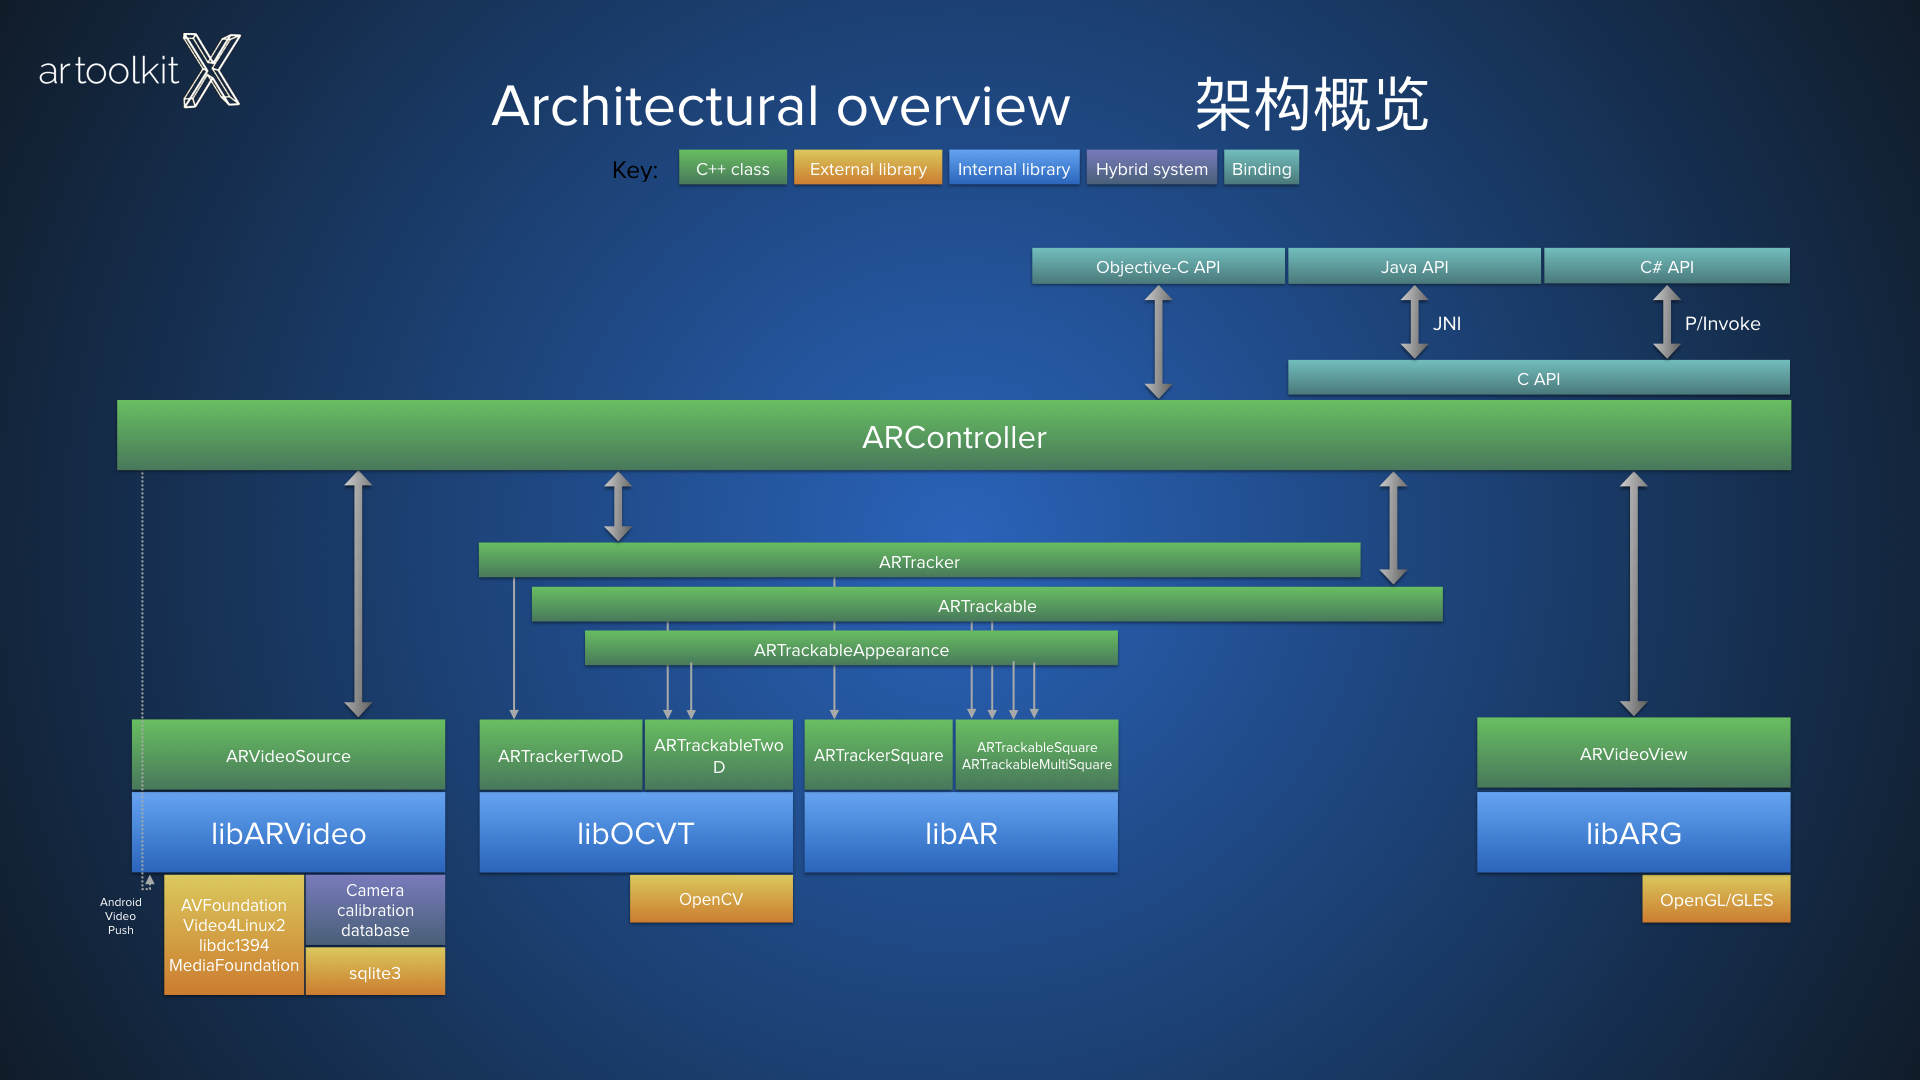
\includegraphics[width=0.8\textwidth]{Abbildungen/artoolkitx-architecture.png}
\caption[ARToolKitX Architektur]{Ein Überblick über die Architektur von ARToolKitX. (Quelle: \cite{artoolkitx:architecture})}
\label{fig:artoolkitx-architecture}
\end{figure}
Grundlegend besteht ARToolKitX aus einer Reihe an C++ Klassen, mit Schnittstellen zu den verschiedenen Programmiersprachen (vergleiche Abbildung \ref{fig:artoolkitx-architecture}).

\subsubsection{Relevanz für diese Arbeit}
ARToolKitX stellt eine moderne und sehr bekannte Tracking-Bibliothek dar, die im Rahmen dieser Arbeit zur Umsetzung der Augmented Reality genutzt werden kann. Des weiteren stellt sie auch eine Beispielanwendung zur Verfügung, die bereits die grundlegenden Konzepte der Augmented Reality implementiert und auf die diese Arbeit aufbauen könnte


\section{Beispielhafte Anwendungen}
Im folgenden wird einmal eine weitere konkrete Anwendung betrachtet, die bereits in der Praxis eingesetzt wird. Im Laufe der Arbeit muss eine Abgrenzung von dieser Lösung erfolgen.

\subsection{Atlas der Humananatomie}\label{sec:atlas-humananatomie}
Visible Body stellt mit der Anwendung \glqq Atlas der Humananatomie 2020\grqq{} eine Anwendung zur Visualisierung von anatomischen Modellen bereit. \todo{zitieren?} Diese steht auch Studenten der Universität Oldenburg über den Bibliothekszugang zur Verfügung und kommt im medizinischen Bereich zum Einsatz. \\
\subsubsection{Anwendung}
Innerhalb der Applikation stehen dem Nutzer verschiedene anatomische Modelle zur Auswahl. Wird eines dieser Modelle ausgewählt wird es zunächst vor einem eintönigen Hintergrund angezeigt. Allerdings besteht zusätzlich die Möglichkeit das Modell im Augmented Reality Bereich darzustellen (siehe \ref{fig:atlas-skelett)}. \\
Mit Hilfe von Gesten kann der Nutzer mit dem Modell interagieren.
\begin{figure}[h!]
\centering
\includegraphics[width=0.8\textwidth]{Abbildungen/app-atlas-skelett.png}
\caption[Atlas der Humananatomie]{Die Darstellung des menschlichen Skeletts in der Anwendung \glqq Atlas der Humananatomie 2020\grqq . (Quelle: Screenshot aus der Anwendung \glqq Atlas der Humananatomie 2020\grqq )}
\label{fig:atlas-skelett}
\end{figure}
